%%%%
%% TEMPLATE HW4 2017-2018
%%%%

\documentclass[addpoints,10pt,answers]{exam}
\usepackage{enumerate}
\usepackage{mathtools}
\usepackage{blkarray}
\usepackage{tikz}
%%%%
% IMPORTANT: YOU SHOULD INSTANTIATE THE FOLLOWING THREE COMMANDS WITH YOUR OWN INFORMATION
\newcommand{\studentonename}{Naldi Gega}     %%% Student one: first and last name
\newcommand{\studentonenumber}{S3154416}  %%% Student one: student number
\newcommand{\studenttwoname}{Emmanouil Gionanidis}     %%% Student two: first and last name
\newcommand{\studenttwonumber}{S3542068}  %%% Student two: student number
\newcommand{\ourdsgroup}{29}         %%% The number of your DS group in Nestor
%%%%

\DeclarePairedDelimiter\abs{\lvert}{\rvert}%


%%%% DO NOT MODIFY 
\newcommand{\hwn}{4}
\pagestyle{headandfoot}
\runningheadrule
\firstpageheader{Discrete Structures (2017-18)}{{\textbf{Answers to Homework No. \hwn}}}{\today}
\runningheader{Discrete Structures (2017-18)}
              {DS Group No.~\ourdsgroup~---~HW\hwn}
              {Page \thepage\ of \numpages}
\firstpagefooter{}{}{}
\runningfooter{}{}{}
 
  \begin{document}
 \boxedpoints
\begin{center}
  \fbox{\fbox{\parbox{5.9in}{\centering
  {\large
  \studentonename~(\studentonenumber) \& \studenttwoname~(\studenttwonumber)  \\
  DS Group No.~\ourdsgroup  }}}
 }
\end{center}
%%%% DO NOT MODIFY  


\begin{questions}

%%%%%%%%%%%%%%%%%%%%%%%%%%%%%%%%%%%%%%%%%%%%%%%%%%%%%%%
\question Question 1:
%%% INSERT YOUR SOLUTIONS HERE
%%%%>>>>>>>>>>>>>>>>>>>>>>>>>>>>>>>>>>
\begin{solution}
\par If we consider a symmetric connected relation as a nonempty connected graph, then we can assume that it has a spanning tree. \\\\
Proof:\\\\
Let G = (V,E) be a nonempty connected graph. We'll show by induction on $\abs{E}$ that G has a spanning tree. The base case is $\abs{E}$ = $\abs{V}-1$ (the least value for which G can be connected); then G itself is a tree . For larger $\abs{E}$, a theorem gives that G contains a cycle. Let uv be any edge on the cycle, and consider the graph G-uv; this graph is connected (since we can route any path that used to go through uv around the other edges of the cycle) and has fewer edges than G, so by the induction hypothesis there is some spanning tree T of G-uv. But then T also spans G, so we are done. 
\end{solution}
%%%%<<<<<<<<<<<<<<<<<<<<<<<<<<<<<<<<<<
%%%%%%%%%%%%%%%%%%%%%%%%%%%%%%%%%%%%%%%%%%%%%%%%%%%%%%%


%%%%%%%%%%%%%%%%%%%%%%%%%%%%%%%%%%%%%%%%%%%%%%%%%%%%%%%
\question Question 2:
%%% INSERT YOUR SOLUTIONS HERE
%%%%>>>>>>>>>>>>>>>>>>>>>>>>>>>>>>>>>>
\begin{solution}
Kruskal’s Algorithm\\
The following algorithm computes a minimal spanning tree:\\
1. Color all vertices yellow\\
2. Color an edge of minimum weight red\\
3. For non red edges e in order of\\ increasing weight:
If the red graph augmented with the edge e remains acyclic, then
color e red and the corresponding vertices black.\\\\
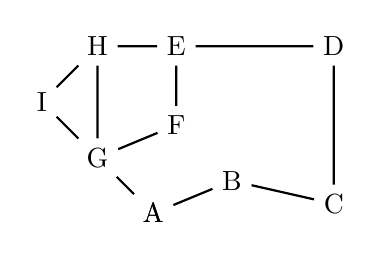
\begin{tikzpicture}
\node (h) at (0,0) {H};
\node [right  of=h] (e)  {E};
\node [below  of=e] (f)  {F};
\node [below left of=h] (i)  {I};
\node [below right  of=i] (g)  {G};
\node [below right of=g] (a)  {A};
\node [below right of=f] (b)  {B};
\node [right of=e] (ed)  {};
\node [right of=ed] (d)  {D};
\node [below right of=g] (a)  {A};
\node [below of=d] (dc)  {};
\node [below of=dc] (c)  {C};
\draw [black,  thick] (e) -- (f) -- (g) -- (h) -- (i) -- (g) -- (a) -- (b) -- (c) -- (d) -- (e) -- (h);
\end{tikzpicture}\\
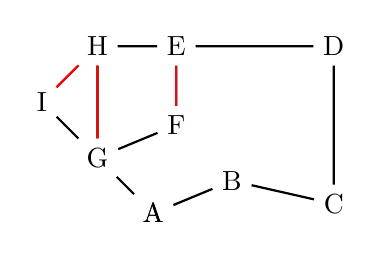
\begin{tikzpicture}
\node (h) at (0,0) {H};
\node [right  of=h] (e)  {E};
\node [below  of=e] (f)  {F};
\node [below left of=h] (i)  {I};
\node [below right  of=i] (g)  {G};
\node [below right of=g] (a)  {A};
\node [below right of=f] (b)  {B};
\node [right of=e] (ed)  {};
\node [right of=ed] (d)  {D};
\node [below right of=g] (a)  {A};
\node [below of=d] (dc)  {};
\node [below of=dc] (c)  {C};
\draw [black,  thick] (e) -- (f) -- (g) -- (h) -- (i) -- (g) -- (a) -- (b) -- (c) -- (d) -- (e) -- (h);
\draw [red,  thick] (i) -- (h)--(g);
\draw [red,  thick] (e) -- (f);
\end{tikzpicture}\\
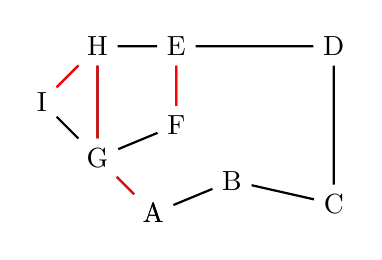
\begin{tikzpicture}
\node (h) at (0,0) {H};
\node [right  of=h] (e)  {E};
\node [below  of=e] (f)  {F};
\node [below left of=h] (i)  {I};
\node [below right  of=i] (g)  {G};
\node [below right of=g] (a)  {A};
\node [below right of=f] (b)  {B};
\node [right of=e] (ed)  {};
\node [right of=ed] (d)  {D};
\node [below right of=g] (a)  {A};
\node [below of=d] (dc)  {};
\node [below of=dc] (c)  {C};
\draw [black,  thick] (e) -- (f) -- (g) -- (h) -- (i) -- (g) -- (a) -- (b) -- (c) -- (d) -- (e) -- (h);
\draw [red,  thick] (i) -- (h)--(g);
\draw [red,  thick] (e) -- (f);
\draw [red,  thick] (g) -- (a);
\end{tikzpicture}\\
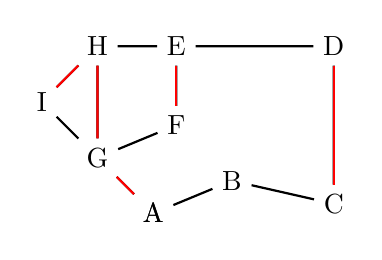
\begin{tikzpicture}
\node (h) at (0,0) {H};
\node [right  of=h] (e)  {E};
\node [below  of=e] (f)  {F};
\node [below left of=h] (i)  {I};
\node [below right  of=i] (g)  {G};
\node [below right of=g] (a)  {A};
\node [below right of=f] (b)  {B};
\node [right of=e] (ed)  {};
\node [right of=ed] (d)  {D};
\node [below right of=g] (a)  {A};
\node [below of=d] (dc)  {};
\node [below of=dc] (c)  {C};
\draw [black,  thick] (e) -- (f) -- (g) -- (h) -- (i) -- (g) -- (a) -- (b) -- (c) -- (d) -- (e) -- (h);
\draw [red,  thick] (i) -- (h)--(g);
\draw [red,  thick] (e) -- (f);
\draw [red,  thick] (g) -- (a);
\draw [red,  thick] (d) -- (c);
\end{tikzpicture}\\
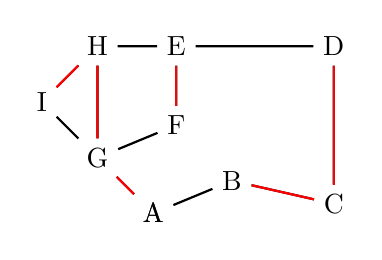
\begin{tikzpicture}
\node (h) at (0,0) {H};
\node [right  of=h] (e)  {E};
\node [below  of=e] (f)  {F};
\node [below left of=h] (i)  {I};
\node [below right  of=i] (g)  {G};
\node [below right of=g] (a)  {A};
\node [below right of=f] (b)  {B};
\node [right of=e] (ed)  {};
\node [right of=ed] (d)  {D};
\node [below right of=g] (a)  {A};
\node [below of=d] (dc)  {};
\node [below of=dc] (c)  {C};
\draw [black,  thick] (e) -- (f) -- (g) -- (h) -- (i) -- (g) -- (a) -- (b) -- (c) -- (d) -- (e) -- (h);
\draw [red,  thick] (i) -- (h)--(g);
\draw [red,  thick] (e) -- (f);
\draw [red,  thick] (g) -- (a);
\draw [red,  thick] (d) -- (c);
\draw [red,  thick] (b) -- (c);
\end{tikzpicture}\\
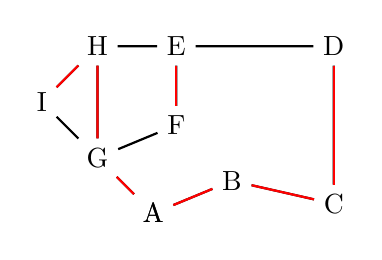
\begin{tikzpicture}
\node (h) at (0,0) {H};
\node [right  of=h] (e)  {E};
\node [below  of=e] (f)  {F};
\node [below left of=h] (i)  {I};
\node [below right  of=i] (g)  {G};
\node [below right of=g] (a)  {A};
\node [below right of=f] (b)  {B};
\node [right of=e] (ed)  {};
\node [right of=ed] (d)  {D};
\node [below right of=g] (a)  {A};
\node [below of=d] (dc)  {};
\node [below of=dc] (c)  {C};
\draw [black,  thick] (e) -- (f) -- (g) -- (h) -- (i) -- (g) -- (a) -- (b) -- (c) -- (d) -- (e) -- (h);
\draw [red,  thick] (i) -- (h)--(g);
\draw [red,  thick] (e) -- (f);
\draw [red,  thick] (g) -- (a);
\draw [red,  thick] (d) -- (c);
\draw [red,  thick] (b) -- (c);
\draw [red,  thick] (b) -- (a);
\end{tikzpicture}\\
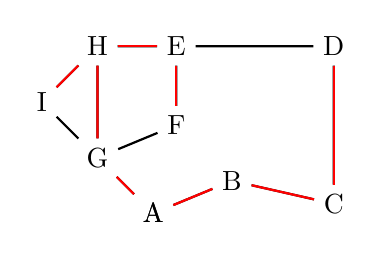
\begin{tikzpicture}
\node (h) at (0,0) {H};
\node [right  of=h] (e)  {E};
\node [below  of=e] (f)  {F};
\node [below left of=h] (i)  {I};
\node [below right  of=i] (g)  {G};
\node [below right of=g] (a)  {A};
\node [below right of=f] (b)  {B};
\node [right of=e] (ed)  {};
\node [right of=ed] (d)  {D};
\node [below right of=g] (a)  {A};
\node [below of=d] (dc)  {};
\node [below of=dc] (c)  {C};
\draw [black,  thick] (e) -- (f) -- (g) -- (h) -- (i) -- (g) -- (a) -- (b) -- (c) -- (d) -- (e) -- (h);
\draw [red,  thick] (i) -- (h)--(g);
\draw [red,  thick] (e) -- (f);
\draw [red,  thick] (g) -- (a);
\draw [red,  thick] (d) -- (c);
\draw [red,  thick] (b) -- (a);
\draw [red,  thick] (b) -- (c);
\draw [red,  thick] (h) -- (e);
\end{tikzpicture}\\
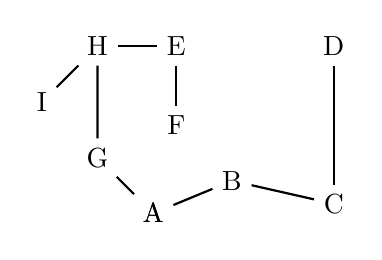
\begin{tikzpicture}
\node (h) at (0,0) {H};
\node [right  of=h] (e)  {E};
\node [below  of=e] (f)  {F};
\node [below left of=h] (i)  {I};
\node [below right  of=i] (g)  {G};
\node [below right of=g] (a)  {A};
\node [below right of=f] (b)  {B};
\node [right of=e] (ed)  {};
\node [right of=ed] (d)  {D};
\node [below right of=g] (a)  {A};
\node [below of=d] (dc)  {};
\node [below of=dc] (c)  {C};
\draw [black,  thick] (i) -- (h)--(g);
\draw [black,  thick] (e) -- (f);
\draw [black,  thick] (g) -- (a);
\draw [black,  thick] (d) -- (c);
\draw [black,  thick] (b) -- (a);
\draw [black,  thick] (b) -- (c);
\draw [black,  thick] (h) -- (e);
\end{tikzpicture}\\
i - h , h - g , e - f = 2  g - a = 3  d - c = 4  c - b = 5  b - a = 6  e - h = 7\\
the weight of the final graph is 2+2+2+3+4+5+6+7=31
\end{solution}
%%%%<<<<<<<<<<<<<<<<<<<<<<<<<<<<<<<<<<
%%%%%%%%%%%%%%%%%%%%%%%%%%%%%%%%%%%%%%%%%%%%%%%%%%%%%%%


%%%%%%%%%%%%%%%%%%%%%%%%%%%%%%%%%%%%%%%%%%%%%%%%%%%%%%%
\question Question 3:
%%% INSERT YOUR SOLUTIONS HERE
%%%%>>>>>>>>>>>>>>>>>>>>>>>>>>>>>>>>>>
\begin{solution}
a)Prim’s Algorithm\\
The following algorithm computes a minimal spanning tree:
1. Color all vertices yellow\\
2. Color an arbitrary vertex black\\
3. As long as there are yellow nodes:\\
(a) Let e be an edge of minimal weight connecting a black vertex with a
yellow vertex.\\
(b) Color e red and the corresponding yellow vertex black\\\\
The following algorithm computes a maximal spanning tree:
1. Color all vertices yellow\\
2. Color an arbitrary vertex black\\
3. As long as there are yellow nodes:\\
(a) Let e be an edge of maximal weight connecting a black vertex with a
yellow vertex.\\
(b) Color e red and the corresponding yellow vertex black\\
b)\\
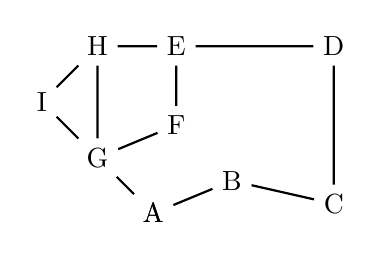
\begin{tikzpicture}
\node (h) at (0,0) {H};
\node [right  of=h] (e)  {E};
\node [below  of=e] (f)  {F};
\node [below left of=h] (i)  {I};
\node [below right  of=i] (g)  {G};
\node [below right of=g] (a)  {A};
\node [below right of=f] (b)  {B};
\node [right of=e] (ed)  {};
\node [right of=ed] (d)  {D};
\node [below right of=g] (a)  {A};
\node [below of=d] (dc)  {};
\node [below of=dc] (c)  {C};
\draw [black,  thick] (e) -- (f) -- (g) -- (h) -- (i) -- (g) -- (a) -- (b) -- (c) -- (d) -- (e) -- (h);
\end{tikzpicture}\\
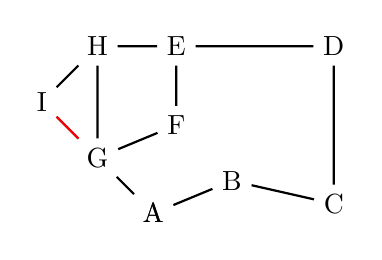
\begin{tikzpicture}
\node (h) at (0,0) {H};
\node [right  of=h] (e)  {E};
\node [below  of=e] (f)  {F};
\node [below left of=h] (i)  {I};
\node [below right  of=i] (g)  {G};
\node [below right of=g] (a)  {A};
\node [below right of=f] (b)  {B};
\node [right of=e] (ed)  {};
\node [right of=ed] (d)  {D};
\node [below right of=g] (a)  {A};
\node [below of=d] (dc)  {};
\node [below of=dc] (c)  {C};
\draw [black,  thick] (e) -- (f) -- (g) -- (h) -- (i) -- (g) -- (a) -- (b) -- (c) -- (d) -- (e) -- (h);
\draw [red,  thick] (i) -- (g);
\end{tikzpicture}\\
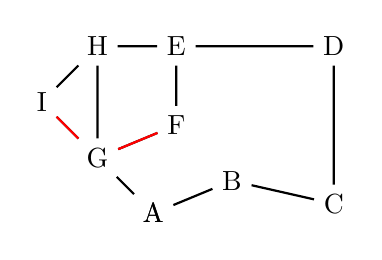
\begin{tikzpicture}
\node (h) at (0,0) {H};
\node [right  of=h] (e)  {E};
\node [below  of=e] (f)  {F};
\node [below left of=h] (i)  {I};
\node [below right  of=i] (g)  {G};
\node [below right of=g] (a)  {A};
\node [below right of=f] (b)  {B};
\node [right of=e] (ed)  {};
\node [right of=ed] (d)  {D};
\node [below right of=g] (a)  {A};
\node [below of=d] (dc)  {};
\node [below of=dc] (c)  {C};
\draw [black,  thick] (e) -- (f) -- (g) -- (h) -- (i) -- (g) -- (a) -- (b) -- (c) -- (d) -- (e) -- (h);
\draw [red,  thick] (i) -- (g);
\draw [red,  thick] (f) -- (g);
\end{tikzpicture}\\
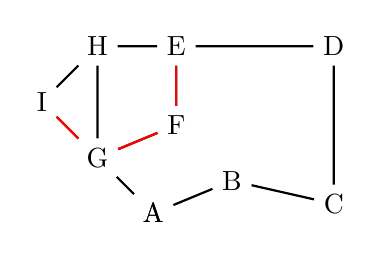
\begin{tikzpicture}
\node (h) at (0,0) {H};
\node [right  of=h] (e)  {E};
\node [below  of=e] (f)  {F};
\node [below left of=h] (i)  {I};
\node [below right  of=i] (g)  {G};
\node [below right of=g] (a)  {A};
\node [below right of=f] (b)  {B};
\node [right of=e] (ed)  {};
\node [right of=ed] (d)  {D};
\node [below right of=g] (a)  {A};
\node [below of=d] (dc)  {};
\node [below of=dc] (c)  {C};
\draw [black,  thick] (e) -- (f) -- (g) -- (h) -- (i) -- (g) -- (a) -- (b) -- (c) -- (d) -- (e) -- (h);
\draw [red,  thick] (i) -- (g);
\draw [red,  thick] (f) -- (g);
\draw [red,  thick] (f) -- (e);
\end{tikzpicture}\\
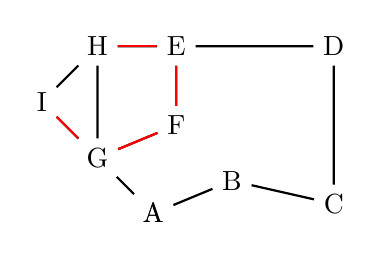
\begin{tikzpicture}
\node (h) at (0,0) {H};
\node [right  of=h] (e)  {E};
\node [below  of=e] (f)  {F};
\node [below left of=h] (i)  {I};
\node [below right  of=i] (g)  {G};
\node [below right of=g] (a)  {A};
\node [below right of=f] (b)  {B};
\node [right of=e] (ed)  {};
\node [right of=ed] (d)  {D};
\node [below right of=g] (a)  {A};
\node [below of=d] (dc)  {};
\node [below of=dc] (c)  {C};
\draw [black,  thick] (e) -- (f) -- (g) -- (h) -- (i) -- (g) -- (a) -- (b) -- (c) -- (d) -- (e) -- (h);
\draw [red,  thick] (i) -- (g);
\draw [red,  thick] (f) -- (g);
\draw [red,  thick] (f) -- (e);
\draw [red,  thick] (h) -- (e);
\end{tikzpicture}\\
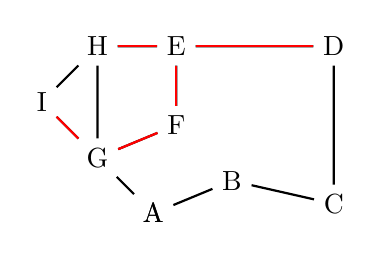
\begin{tikzpicture}
\node (h) at (0,0) {H};
\node [right  of=h] (e)  {E};
\node [below  of=e] (f)  {F};
\node [below left of=h] (i)  {I};
\node [below right  of=i] (g)  {G};
\node [below right of=g] (a)  {A};
\node [below right of=f] (b)  {B};
\node [right of=e] (ed)  {};
\node [right of=ed] (d)  {D};
\node [below right of=g] (a)  {A};
\node [below of=d] (dc)  {};
\node [below of=dc] (c)  {C};
\draw [black,  thick] (e) -- (f) -- (g) -- (h) -- (i) -- (g) -- (a) -- (b) -- (c) -- (d) -- (e) -- (h);
\draw [red,  thick] (i) -- (g);
\draw [red,  thick] (f) -- (g);
\draw [red,  thick] (f) -- (e);
\draw [red,  thick] (h) -- (e);
\draw [red,  thick] (d) -- (e);
\end{tikzpicture}\\
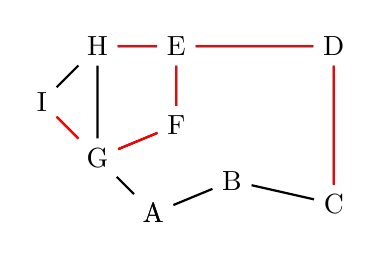
\begin{tikzpicture}
\node (h) at (0,0) {H};
\node [right  of=h] (e)  {E};
\node [below  of=e] (f)  {F};
\node [below left of=h] (i)  {I};
\node [below right  of=i] (g)  {G};
\node [below right of=g] (a)  {A};
\node [below right of=f] (b)  {B};
\node [right of=e] (ed)  {};
\node [right of=ed] (d)  {D};
\node [below right of=g] (a)  {A};
\node [below of=d] (dc)  {};
\node [below of=dc] (c)  {C};
\draw [black,  thick] (e) -- (f) -- (g) -- (h) -- (i) -- (g) -- (a) -- (b) -- (c) -- (d) -- (e) -- (h);
\draw [red,  thick] (i) -- (g);
\draw [red,  thick] (f) -- (g);
\draw [red,  thick] (f) -- (e);
\draw [red,  thick] (h) -- (e);
\draw [red,  thick] (d) -- (e);
\draw [red,  thick] (d) -- (c);
\end{tikzpicture}\\
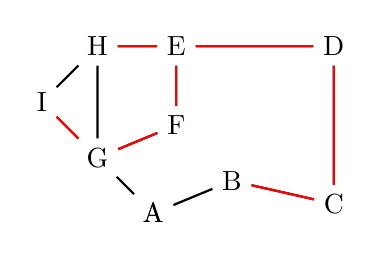
\begin{tikzpicture}
\node (h) at (0,0) {H};
\node [right  of=h] (e)  {E};
\node [below  of=e] (f)  {F};
\node [below left of=h] (i)  {I};
\node [below right  of=i] (g)  {G};
\node [below right of=g] (a)  {A};
\node [below right of=f] (b)  {B};
\node [right of=e] (ed)  {};
\node [right of=ed] (d)  {D};
\node [below right of=g] (a)  {A};
\node [below of=d] (dc)  {};
\node [below of=dc] (c)  {C};
\draw [black,  thick] (e) -- (f) -- (g) -- (h) -- (i) -- (g) -- (a) -- (b) -- (c) -- (d) -- (e) -- (h);
\draw [red,  thick] (i) -- (g);
\draw [red,  thick] (f) -- (g);
\draw [red,  thick] (f) -- (e);
\draw [red,  thick] (h) -- (e);
\draw [red,  thick] (d) -- (e);
\draw [red,  thick] (d) -- (c);
\draw [red,  thick] (b) -- (c);
\end{tikzpicture}\\
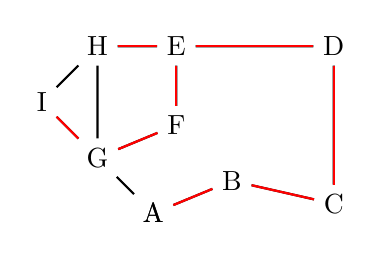
\begin{tikzpicture}
\node (h) at (0,0) {H};
\node [right  of=h] (e)  {E};
\node [below  of=e] (f)  {F};
\node [below left of=h] (i)  {I};
\node [below right  of=i] (g)  {G};
\node [below right of=g] (a)  {A};
\node [below right of=f] (b)  {B};
\node [right of=e] (ed)  {};
\node [right of=ed] (d)  {D};
\node [below right of=g] (a)  {A};
\node [below of=d] (dc)  {};
\node [below of=dc] (c)  {C};
\draw [black,  thick] (e) -- (f) -- (g) -- (h) -- (i) -- (g) -- (a) -- (b) -- (c) -- (d) -- (e) -- (h);
\draw [red,  thick] (i) -- (g);
\draw [red,  thick] (f) -- (g);
\draw [red,  thick] (f) -- (e);
\draw [red,  thick] (h) -- (e);
\draw [red,  thick] (d) -- (e);
\draw [red,  thick] (d) -- (c);
\draw [red,  thick] (b) -- (c);
\draw [red,  thick] (b) -- (a);
\end{tikzpicture}\\
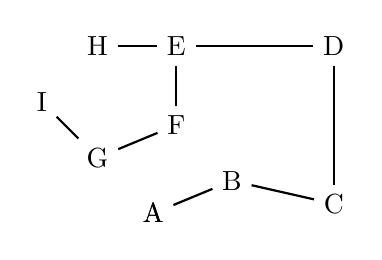
\begin{tikzpicture}
\node (h) at (0,0) {H};
\node [right  of=h] (e)  {E};
\node [below  of=e] (f)  {F};
\node [below left of=h] (i)  {I};
\node [below right  of=i] (g)  {G};
\node [below right of=g] (a)  {A};
\node [below right of=f] (b)  {B};
\node [right of=e] (ed)  {};
\node [right of=ed] (d)  {D};
\node [below right of=g] (a)  {A};
\node [below of=d] (dc)  {};
\node [below of=dc] (c)  {C};
\draw [black,  thick] (i) -- (g);
\draw [black,  thick] (f) -- (g);
\draw [black,  thick] (f) -- (e);
\draw [black,  thick] (h) -- (e);
\draw [black,  thick] (d) -- (e);
\draw [black,  thick] (d) -- (c);
\draw [black,  thick] (b) -- (c);
\draw [black,  thick] (b) -- (a);
\end{tikzpicture}\\
The weight is 3+8+2+7+8+4+5+6=41
\end{solution}
%%%%<<<<<<<<<<<<<<<<<<<<<<<<<<<<<<<<<<
%%%%%%%%%%%%%%%%%%%%%%%%%%%%%%%%%%%%%%%%%%%%%%%%%%%%%%%


%%%%%%%%%%%%%%%%%%%%%%%%%%%%%%%%%%%%%%%%%%%%%%%%%%%%%%%
\question Question 4:
%%% INSERT YOUR SOLUTIONS HERE
%%%%>>>>>>>>>>>>>>>>>>>>>>>>>>>>>>>>>>
\begin{solution}
\\1)\\
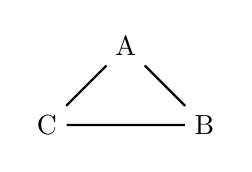
\begin{tikzpicture}
\node (a) at (0,0) {A};
\node [below  of=a] (m)  {};
\node [right  of=m] (b)  {B};
\node [left  of=m] (c)  {C};
\draw [black,  thick] (b) -- (a)--(c)--(b);
\end{tikzpicture}\\
The above graph is regular because all vertices have the same degree of 2, it is connected because there is a path from any vertex to any vertex but it is not complete because there are loops.\\
2)\\
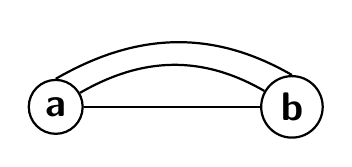
\begin{tikzpicture}[->,auto,node distance=3cm,
  thick,main node/.style={circle,draw,font=\sffamily\Large\bfseries}]
\node[main node] (1) {a};
\node[main node] (2) [right of=1] {b};
\draw [-] (1) -- (2);
\draw [-] (2) to [out=150,in=30] (1);
\draw [-] (2.north) to [out=150,in=30] (1.north);
\end{tikzpicture}\\
The above graph is regular because all vertices have the same degree, it is not complete because it has parallel edges and all vertices have degree 3.
\end{solution}
%%%%<<<<<<<<<<<<<<<<<<<<<<<<<<<<<<<<<<
%%%%%%%%%%%%%%%%%%%%%%%%%%%%%%%%%%%%%%%%%%%%%%%%%%%%%%%


%%%%%%%%%%%%%%%%%%%%%%%%%%%%%%%%%%%%%%%%%%%%%%%%%%%%%%%
\question Question 5:
%%% INSERT YOUR SOLUTIONS HERE
%%%%>>>>>>>>>>>>>>>>>>>>>>>>>>>>>>>>>>
\begin{solution}
A Hamiltonian path in a graph visits each vertex exactly once.\\
One path of the graph is: H, E, A, D, F, G, C, B \\
And another one is: B, C, G, F, D, A, E, H
\end{solution}
%%%%<<<<<<<<<<<<<<<<<<<<<<<<<<<<<<<<<<
%%%%%%%%%%%%%%%%%%%%%%%%%%%%%%%%%%%%%%%%%%%%%%%%%%%%%%%


%%%%%%%%%%%%%%%%%%%%%%%%%%%%%%%%%%%%%%%%%%%%%%%%%%%%%%%
\question Question 6:
%%% INSERT YOUR SOLUTIONS HERE
%%%%>>>>>>>>>>>>>>>>>>>>>>>>>>>>>>>>>>
\begin{solution}
\\
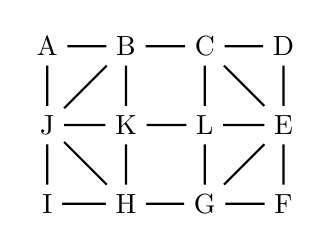
\begin{tikzpicture}
\node (a) at (0,0) {A};
\node [right  of=a] (b)  {B};
\node [right  of=b] (c)  {C};
\node [right  of=c] (d)  {D};
\node [below  of=a] (j)  {J};
\node [right  of=j] (k)  {K};
\node [right  of=k] (l)  {L};
\node [right  of=l] (e)  {E};
\node [below  of=j] (i)  {I};
\node [right  of=i] (h)  {H};
\node [right  of=h] (g)  {G};
\node [right  of=g] (f)  {F};
\draw [black,  thick] (j) -- (i) -- (h) -- (g) -- (f) -- (e) -- (d) -- (c) -- (b) -- (a) -- (j) -- (k) -- (h) -- (j) -- (b) -- (k) -- (l) -- (e) -- (g) -- (l) -- (c) -- (e);
\end{tikzpicture}\\
After traversing J, H, G, F, E, D, C, B, A, J, K, H, J, B, K we cannot go to L because the edge K-L is a bridge and cannot be removed.
\end{solution}
%%%%<<<<<<<<<<<<<<<<<<<<<<<<<<<<<<<<<<
%%%%%%%%%%%%%%%%%%%%%%%%%%%%%%%%%%%%%%%%%%%%%%%%%%%%%%%


\end{questions}
\end{document}